\chapter{Mechanical and hydrologic properties of Whillans ice \\stream till: Implications for basal strength \\and stick-slip failure}

\section{Abstract}
Ice streams transport large volumes of inland ice to the ocean and play a key role in the mass balance of the Antarctic ice sheet. The rate and style of ice stream basal slip are governed, in part, by the underlying till whose physical properties are poorly constrained. To address this problem, we conducted a suite of laboratory measurements to document the permeability, stiffness, consolidation behavior, and compressional wave speeds of Whillans Ice Stream till samples. We investigated the effects of stepped and cyclic loading on the evolution of the till. Initial permeabilities were 3.8-4.9�10-17 m2 (porosities 28.1-31.8\%), which decreased to 2.0�10-19 m2 (20.4\%) at 10 MPa effective stress. P-wave velocities span from 2.26-3 km/s over this effective stress range, and are well described by an effective medium model. The laboratory measurements were used to parameterize a 1-D numerical model to predict the till?s response to stress perturbations. Perturbations corresponding to tidal periods produce a drained and strengthened layer tens of cm thick. For perturbations over timescales of weeks to months, as expected for till motion over basement features, the drained zone is a few meters thick. This strong layer can become brittle upon unloading, and may facilitate observed stick-slip motion. Extrapolation of our effective medium model suggests low basal effective stresses, on the order of a few tens of kPa, are needed to produce seismic velocities observed in the field (Vp ~1750 m/s; Vs ~160 m/s), and provides an approach to quantify and monitor in situ conditions.

\section{Introduction}
Ice streams are regions of fast-moving grounded ice shearing past slower-moving regions of ice.  In Antarctica, ice streams discharge over 90\% of the interior accumulation over only ~13\% of the coastline, making them critical to the ice sheet mass balance [Morgan et al., 1982]. Motion of ice streams is complex, as the flow can migrate, stagnate, or even occur in a stick-slip fashion, inducing seismicity [Anandakrishnan et al., 2003; Wiens et al., 2008; Walter et al., 2011]. Many models have attempted to explain the nature of ice stream movement, mostly invoking high basal water pressures, often coupled to soft subglacial sediments that smooth the bed and deform to lubricate motion [Bentley, 1987; Alley et al., 2004; Cuffey and Paterson, 2010]. However, direct measurements sampling the subglacial environment of ice streams remain highly limited [Cuffey and Paterson, 2010].

Ice streaming is often observed to start over sedimentary basins, suggesting that flow begins where the bed first becomes deformable [Anandakrishnan et al., 1998; Bell et al., 1998; Cuffey and Paterson, 2010]. Understanding the mechanical properties of the till immediately underlying the ice is therefore of primary importance, as it may control the flow rate and stability of the ice stream, and ultimately play a key role in the ice sheet mass balance [Tulaczyk et al., 2000; Kamb, 2001]. Sediment-water interactions are also important in controlling grounding zone processes [e.g. Dowdeswell et al., 2008; Cowan et al., 2014].

Laboratory till-deformation experiments have provided important insights into the rheologic behavior of till [Clarke, 1987; Iverson et al., 1997; 1998; Kavanaugh and Clarke, 2006; e.g. Thomason and Iverson, 2008; Iverson and Zoet, 2015], and the measured mechanical properties are comparable to the few reported field measurements, suggesting that the lab measurements can be upscaled effectively [Tulaczyk, 2006]. Since that important earlier work, there has been an increasing interest in the response of till to cyclic loading because of a growing body of evidence indicating that ice stream motion is tidally modulated in many cases. Examples include variations in velocity observed on Kamb Ice Stream (formerly ice stream C) [Anandakrishnan and Alley, 1997], on neighboring Bindschadler Ice Stream (formerly ice stream D) [Anandakrishnan et al., 2003], and elsewhere [Gudmundsson, 2007; Zoet et al., 2012].  Water-pressure observations beneath Whillans and Kamb Ice Streams also documented diurnal variations of 10-20 kPa, consistent with the dominant tidal frequency in the region [Engelhardt and Kamb, 1997; Kamb, 2001]. 

The downglacier part of Whillans Ice Stream exhibits two seismic motion events per day that are tightly linked to the tide, occurring just after high tide and just before low tide [Bindschadler et al., 2003; Winberry et al., 2014]. Walker et al. [2013] proposed that the rising tide beneath an adjacent ice shelf causes downward bending extending a few ice thicknesses inland, compacting till beneath; the falling tide is then hypothesized to cause upwarp that may pump ocean water upglacier into the grounded flexural zone.  The cyclic loading, with expected amplitude on the order of 50 kPa, leads to the development of ?sticky spots? or asperities with higher shear strength and stiffness than the surrounding material, which promote the observed repeated stick-slip failure [Winberry et al., 2011; Pratt et al., 2014; Winberry et al., 2014; Walter et al., 2015]. Features observed near the grounding zone of Whillans Ice Stream, including upwarped surface topography, folded internal reflectors that indicate increased basal drag, and water/sediment exchange at the grounding line, are consistent with flexural behavior producing sticky spots through till compaction [Christianson et al., 2013; Horgan et al., 2013].  

This prior work leads to a conceptual model wherein the interplay of material properties and time-dependent hydraulic processes produces a layer of till sufficiently stiff to support brittle stick-slip failure. Till hydrologic and consolidation properties ultimately govern the time scales of pore pressure diffusion and drainage [Tulaczyk et al., 2000], which are central to the proposed tidal pumping mechanism, and also to hypothesized mechanisms of till weakening through generation of high pressures in front of ploughed debris [Thomason and Iverson, 2008]. Here, we report on a suite of tri-axial deformation experiments on till from beneath Whillans Ice Stream that include measurements of porosity, permeability, stiffness, and acoustic velocity under both stepped and cyclic loading conditions, aimed at understanding temporal and spatial scales of drainage-modulated processes in the till. We then incorporate these laboratory data into a transient 1-D model that couples till deformation (consolidation) and drainage to explore the hypothesis that cyclic loading produces a brittle layer that is able to support stick-slip failure. 

\subsection{Geologic Setting}
Whillans Ice Stream, formerly ice stream B, is one of five major ice streams located on the Siple Coast of Western Antarctica (Figure 1). Whillans is considered a fast-flowing ice stream, with over 400 m of surface displacement per year, though its velocity is currently decreasing and it may become stagnant within 100-200 years [Whillans and Van der Veen, 1993; Joughin et al., 2005]. The ice is approximately 1 km thick at the UpB camp, located approximately 400 km from the grounding line, where the ice stream has been most intensively studied [Blankenship et al., 1986; 1987; Rooney et al., 1987; Engelhardt et al., 1990]. The ice flows over several meters of unconsolidated till that lie unconformably over a poorly lithified sedimentary sequence. Temperatures at the ice-till interface are at approximately the pressure melting point of -0.8� C [Engelhardt et al., 1990; Tulaczyk et al., 1998]. A surface slope of 0.0013 � 0.003 provides an average gravitational driving stress of ~ 13-20 kPa [Alley, 1993; Tulaczyk et al., 1998].

Cores of till were obtained at the UpB camp during field seasons from 1989-1993 (Figure 1). This unique suite of samples has been subjected to mechanical testing to measure several geotechnical properties, including texture, composition, and strength as a function of strain, strain rate, and effective stress [Kamb, 1991; Tulaczyk et al., 1998; 2000]. After study, the samples were stored at room conditions (ambient humidity and temperature) by K. Licht at Indiana University-Purdue University Indianapolis and generously made available for this work. During drilling, observed fluid pressures in the borehole were within 50 kPa of the 9 MPa ice overburden (i.e. effective normal stresses less than ~50 kPa and perhaps much less [Tulaczyk et al., 2001]), such that shear stresses at the bed are much less than those required to significantly deform the ice internally. This is consistent with laboratory shearing experiments showing that the cohesion of the tills is generally negligible and their shear strength is only a few kPa under a normal stress of ~9 kPa [Kamb, 1991; 2001]. Such a low shear strength has led to the interpretation that rapid surface displacement of the ice stream is primarily the result of basal processes (sliding between ice and till, ploughing, and till deformation) [Blankenship et al., 1986; 1987; Engelhardt and Kamb, 1997].

\section{Materials and Methods}
\subsection{Sample Preparation}
We tested two samples from the Up-B expedition, obtained from depths of 0.3-0.4 m and 1.6-1.7 m (Samples 1744 and 1754) below the ice-till interface in borehole 89-1-4 (Figure 1). The till in general is a dark-grey unstructured diamicton, consisting of sand, silt, and clay-sized fractions in a bimodal distribution with scattered pebbles [Tulaczyk et al., 1998]. Because the samples were stored at ambient conditions for many years, we used an ultrasonic humidifier with purified water to carefully re-hydrate the intact core samples. The samples were then trimmed into 2.54 cm diameter cylinders with lengths of 2.1 and 2.4 cm, with care taken to subsample only the most undisturbed parts of the core. Initial sample dimensions were recorded before jacketing and testing. The samples, together with end platens and porous frits, were jacketed with heat shrink tube. The shrink jacket was then sealed with tie-wire, and a thicker, stronger confining jacket was applied just over the ends of the specimen and secured with hose-clamps (Figure 2). 

\subsection{Tri-axial Loading}
Samples were loaded into a tri-axial pressure vessel. Confining (radial) and axial stresses were set to be equal in our tests (isostatic stress condition wherein ?1 = ?2 = ?3), and applied via a silicone oil pressurized by a piston syringe pump. Sample pore fluid pressure was controlled at each sample face using two additional high-precision syringe pumps. Prior to deformation, the samples were allowed to equilibrate for 24 hours under a pore pressure of 200 kPa and confining pressure of 300 kPa (effective pressure of 100 kPa) to ensure complete fluid saturation. During the equilibration stage, only one pore fluid pump was used to maintain pore pressure. Pore fluid pumps and the pressure vessel were maintained at a constant temperature of 29.5 � 0.1�C using a temperature chamber that surrounds the apparatus to minimize thermal expansion effects. Both pressure and volume were monitored continuously in both of the pore fluid pumps to a precision of � 1 kPa and � 1 mm3 respectively, to document volumetric strain and changes in sample porosity. 

The final porosity of the sample is obtained by weighing the fully saturated sample immediately after the test, and again after oven drying at 110 �C for 24-48 hours [ASTM D2216]. The difference indicates the mass of interstitial water in the sample, from which the pore fluid volume is defined (assuming a water density of 1000 kg m-3); the total volume of the sample is determined from direct measurements of its dimensions using a micrometer. Using the final porosity value determined by this approach, porosity throughout the experiment is then calculated from the pore fluid pump volume measurements that record sample volume change (i.e. fluid expulsion or uptake).

Two loading paths were used to test the till samples. First, a simple incremental loading path was applied, in which the effective stress was increased step-wise and then allowed to equilibrate in a series of stages. Equilibration was defined as the point when pore volume and sample length were no longer changing significantly. Permeability and acoustic velocity were then measured after equilibration at each load step, as described in detail below. The second testing profile was designed to emulate cyclic loading as is hypothesized to result from tidally-driven ice flexure [Walker et al., 2013]. We achieved this by applying a sequence of sinusoidal loading patterns with a period of 24-hours and amplitudes of 20, 50, 75, and 150 kPa. The amplitude of each sinusoid pattern was maintained for 5-10 days (5-10 cycles), starting with 20 kPa and increasing sequentially. Pore volumes and axial strain were monitored continuously during the tests, and permeability was measured following equilibration after each set of cycles at a given amplitude.

\subsection{Permeability and Compressibility}
The permeability k [m2] of the samples was determined using a steady-state constant-head method. The upstream and downstream pore pressure pumps were held at constant pressures to maintain a pressure gradient across the specimen (ranging from 20-80 kPa in our tests). After reaching a steady-state, defined by equal flow rates in the two pumps to within ~10\%, water flux through the sample was determined from pump volume records (Figure 3). We then computed permeability using Darcy's relation:
(1)	  
where Q is the steady-state flow rate [m3 s-1], ? is the dynamic fluid viscosity  (0.0008 Pas at 29.5�C), L is the sample length [m], A is the cross-sectional area of the sample [m2], and ?P is the difference in pressure between the upstream and downstream pumps [Pa]. For each effective stress step, we conducted permeability tests with three different pressure gradients, and report the permeability as the mean of these values (all data are provided in the Supplementary Materials). 
Sample compressibility, ? [Pa-1], is calculated from the total sample volume change, as recorded in pore-fluid pump volumes, resulting from a known change in effective stress:
(2)  
where V and dV are sample volume and change in sample volume [m3], respectively, and dPe is the increment in effective stress [Pa]. 

\subsection{Acoustic Velocity}
Compressional wave velocity was determined using a time-of-flight technique through the sample, corrected to account for travel time through the end-caps and porous frits [Knuth et al., 2013; Carpenter et al., 2014]. The end-caps used to apply axial load to the sample were equipped with lead-zirconate-titanate (PZT) transducers (Figure 2). A -900 VDC pulse was applied to one (transmitting) transducer, creating a propagating elastic wave with a center frequency of approximately 500 kHz. The signal from a second (receiving) transducer in the opposite end cap was recorded by a high-speed data acquisition system with a resolution of 16-bits over a  1 V range at 50 MHz sampling rate (Figure 4). To reduce noise in individual waveform records, 100 waveforms were recorded and stacked to form one record. This was repeated a minimum of 25 times for each effective stress state. The P-wave arrivals are emergent at low stresses, but can be resolved accurately with a pattern cross-correlation technique, in which a pattern arrival is correlated with measured waveforms and the point of maximum correlation picked as the arrival. Velocity is then calculated from the corrected travel times for the first arrivals, and using directly measured sample length.

Acoustic velocities (both P- and S-wave speeds) in unconsolidated sediments and soils can also be predicted by effective-medium models [e.g. Dvorkin et al., 1999; Helgerud et al., 1999]. Application of such a model can provide a key link between in situ physical properties and conditions, including effective stress and pore-fluid pressure, and borehole or field-based geophysical data. Here we compose an effective-medium model following Dvorkin et al. [1999] (see Appendix for details), incorporating X-Ray Diffraction (XRD) data that define the bulk till mineralogy, and then benchmark the model against our laboratory measurements of P-wave velocity. 

\section{Results}
The initial porosity of both core samples was 28-32\%. This is lower than the estimated in situ porosity of 40\% [Engelhardt et al., 1990], and may be attributed to storage and sampling artifacts. Samples were obtained with a piston corer; the hammering action of the coring process may have compacted the samples from their in situ state. After initial characterization and cataloging, the samples were stored at room temperature and humidity, and may have been subject to pore-space reduction associated with desiccation and matrix suction effects. To inform our effective-medium modeling, we conducted X-ray diffraction analyses on material from the two cores of till from beneath the ice stream that we tested in our deformation experiments (Figure S1). The diffraction patterns from both samples show almost identical mineralogy, with minor background count differences, and indicate that the till consists primarily of clay minerals, with a significant quartz fraction and some feldspar family minerals (Table 1). 

\subsection{Consolidation and Compressibility}
Our stepped loading tests (SAL1744) find a systematic decrease in porosity and concomitant increase in stiffness with increasing effective stress, following a strain-hardening trend typical of soils and sediments [Wood, 1990]. During stepped-loading, the effective confining pressure was increased from 100 kPa to 1 MPa in 100 kPa steps, decreased to 50 kPa, and then increased again (reloaded) to 10 MPa (Figure 5A). Volumetric and axial strain show very similar trends during the entire step loading test. The initial loading stages produced an integrated volumetric strain of about 3\%, which was mostly recovered during unloading. Final strains of 6-10\% were achieved at 10 MPa effective stress (Figure 5B). The initial porosity of the sample was 28.1\% and the initial compressibility was ~5x10-8 Pa-1. At 10 MPa effective stress, the porosity was reduced to 20.4\% and compressibility to 4.8�10-9 Pa-1. Unloading the sample resulted in modest poroelastic rebound to a porosity of 23.6\% (Figure 6B). 
During our cyclic loading tests (SAL1754), strain continued to accumulate with each cycle, even though the effective stresses did not exceed those applied in preceding cycles. The amount of incremental strain decreased asymptotically with each set of cycles at a given amplitude, and then increased sharply after increasing the amplitude of the oscillations (Figures 5C,D, S2). Initial loading produced 0.88\% axial strain. After 10 cycles of 20 kPa, axial strain increased to 0.95\% (corresponding to a porosity of 31.2\%). After 25 cycles of 50 kPa, strain increased asymptotically to 1.04\% (porosity of 31\%); 10 cycles at 75 kPa increased strain to 1.09\% (porosity of 30.5\%). The final 15 cycles at 150 kPa increased the strain to 1.77\% and reduced the porosity to 28.3\%.

\subsection{Permeability}
 Permeability decreased systematically with loading, exhibiting nearly two orders of magnitude decrease upon loading to 10 MPa effective stress. Permeability decreases most rapidly early in the loading history, consistent with porosity loss and strain hardening. The samples had an initial permeability of 3.8�10-17 m2 and 4.9�10-17 m2 at an effective stress of 100 kPa, consistent with values reported for other till samples (1�10-19 m2 to 1�10-13 m2) [Freeze and Cherry, 1979], and slightly lower than values of 2�10-16 m2 reported from large scale field measurements at the Whillans drill site taken by a falling head permeameter [Engelhardt et al., 1990]. We note that the higher permeabilities reported from the field measurements may reflect a component of non-Darcian flow at the ice-till interface. At 1 MPa effective stress (corresponding to 25.3\% porosity), permeability was reduced by a factor of ~15-20, to 2.5�10-18 m2, and recovered only slightly to 3.3�10-18 m2 upon unloading. After loading to 10 MPa effective stress (20.4\% porosity), permeability was reduced to 2.0�10-19 m2 (Figures 6A,B).
The cyclic loading test exhibited about an order of magnitude reduction in permeability over 60 loading cycles, despite the fact that the loading oscillations did not exceed the peak effective stress previously applied to the specimens, consistent with the trends of strain and porosity loss (c.f. Figures 5C-D). After 10 load cycles of 20 kPa (resulting in a porosity of 31.2\%), the permeability of the specimen was reduced by a factor of 1.6, from an initial value of 3.8�10-17 m2 to 2.4�10-17 m2. This was followed by 25 load cycles of 50 kPa (31\% porosity) in which the permeability was reduced to 1.3�10-17 m2. Another 10 cycles of 75 kPa loading reduced the permeability to 1.1�10-17 m2 (30.5\% porosity). The final cycle set consisted of 15 cycles at 150 kPa, and the permeability was reduced to 3.9�10-18 m2 (corresponding to 28.3\% porosity) (Figure 6C,D). 
 
 \subsection{Acoustic Velocity}
 P-wave velocity increased systematically with effective stress in our stepped loading test. At an effective pressure of 0.7 MPa (corresponding to 26.4\% porosity), Vp values of ~2.26 km/s were observed, increasing to nearly 3 km/s at 10 MPa effective stress (20.4\% porosity) (Figure 7A). The compressional wave velocity data from the laboratory are fit reasonably well by our effective medium model, assuming a critical porosity of 40\% and grain contact number of 8 (Table 1; Appendix). Extrapolation of the effective medium model to slightly lower effective stresses predicts that in situ effective stresses <~100 kPa, and in situ porosities >~40\% would be required to produce P and S wave velocities of ~1750 m/s and 160 m/s, respectively, that are observed via field experiments [Blankenship et al., 1986; 1987; Luthra et al., 2016]. This provides new evidence supporting inferences of low effective stresses, and thus low shear strength, at the base of the ice stream (Figure 7). 
 
 \subsection{Hydrologic Model}
 To explore the implications of our laboratory measurements for the hypothesized development of a ?hard layer? that enables stick-slip motion of the ice stream, we developed a simple 1-D transient finite-difference model implemented with the Python package FiPy [Guyer et al., 2009] that simulates coupled compaction and drainage in a vertical column of till with heterogeneous properties (Figure 8). Because permeability and compressibility vary strongly and nonlinearly with effective stress, we use a 0.01 m nodal spacing and a time step of 0.01 - 1000 seconds, increasing as the model changes become more gradual. This allows us to quantify the evolution of till porosity, stiffness, permeability, and effective stress in response to perturbations at the ice stream bed. By incorporating the constitutive relations obtained from our laboratory measurements (Figure S3) we account for the significant and non-linear evolution of porosity, permeability, and compressibility during compaction [Skarbek and Saffer, 2009] that are typically not included in simple models having homogeneous and/or time-invariant physical properties [e.g. Gibson, 1958; Wissa et al., 1971]. 
This model provides first-order insights into the time-dependent behavior of the system and the time and length scales of drainage relevant to subglacial processes. The model is initialized with a hydrostatic pressure gradient, and the vertical effective stress at the top boundary (ice-till interface) is then increased instantaneously to explore the response to a perturbation. This value is then held constant (Dirichlet boundary), and the till layer is allowed to evolve. The bottom boundary, 10 m below the till-ice interface, is controlled with Neumann boundary conditions of zero flux to emulate the harder semi-consolidated bedrock on which the till is deposited. The upper boundary is physically equivalent to allowing drainage into an ice-contact water system at the specified pressure, of the sort known to exist beneath Whillans Ice Stream [Engelhardt and Kamb, 1997; Kamb, 2001].  
The governing equation for fluid flow is:

where h is hydraulic head [m],  is specific storage [m-1], and K is hydraulic conductivity [m s-1]. Specific storage is in turn defined from compressibility, where ?is the till compressibility and ?is the fluid compressibility and  the sample porosity.
(4) 
Hydraulic conductivity is defined from permeability by: 
(5)  
where  is the fluid density [kg m-3], g the acceleration of gravity [m s-2], and  is the fluid viscosity [Pa s]. Porosity, permeability, and compressibility are determined for each model cell from empirical least-squares fits to our experimental data (equations 6-8), and updated at each time step as hydraulic head and effective stress evolve (Figure 8A). The permeability prediction from our empirical fit slightly under predicts observed permeabilities at the highest porosities, but errors are less than a factor of two and inconsequential in the modeling scheme. As the porosity is rapidly reduced during initial drainage, the empirical relation and model quickly converge. The model also provides a minimum estimate of active layer depth due to the slight under prediction of permeability in the early stages of the model run.
(6)  
(7)  
(8)  
For a simple drop in pressure at the top of the till (or equivalently a step increase in pressure within the till caused by mechanical loading), there is initial drainage to the top of the column. The uppermost few cm of the till quickly drains, and as a result its porosity and permeability are significantly reduced and its stiffness increases (Figure 9). This results in self-limited drainage from the top of the layer relative to that predicted for a homogeneous case (i.e. in which the till properties are time invariant) [Wissa et al., 1971], and leads to the development of a thin zone at the top of the till where consolidation has progressed. This zone is characterized by increased effective vertical stress (and thus increased shear strength), increased stiffness, and decreased porosity (Figure 9). As the till layer responds and drains, a minimum in vertical effective stress, and in shear strength, propagates downward. Over timescales of tidally-driven perturbations, this minimum in strength reaches approximately 0.7 m; by 30 days it propagates to ~4 m. Upon unloading, during upward flexure of the ice, the till is in an overconsolidated state and has become embrittled [Wood, 1990], possibly promoting seismogenic failure.
 
 \section{Discussion}
 Despite the fact that samples were stored at room conditions for a number of years, we expect their properties to be representative of in-situ conditions. Once rehydrated during sample carving, then saturated in the pressure vessel and loaded to effective stresses of ~100 kPa the properties should track undisturbed samples. Our observations of systematic behaviors and trends as well as generally low permeability measurements suggest that any permanent effects from dry storage are negligible. In fact, it is likely that piston coring had a larger effect that desiccation on the sample properties.
 
 \subsection{Till physical properties and relevance to sticky spot development}
 The evolution of porosity, permeability, and stiffness observed in our experiments is consistent with the conceptual model of a hard layer of till that enables stick-slip behavior. For example, during compaction in our experiments, till compressibility was reduced by a factor of 7 from an initial value of 7�10-8 Pa-1. We also observed that when subjected to load cycling, the till progressively compacts as a result of small-amplitude fluctuations in stress, even if the effective stresses never exceed values previously experienced by the material. These processes are likely to be increasingly important near the grounding line, where ice flexure due to ocean tides is continually changing the stress state at the base of the ice and possibly produces persistent brittle layers of till. 
Drainage times obtained from the 1-D hydrological model are also consistent with this conceptual model. In a 12 hour tidal period a compacted zone a few tens of centimeters thick can form. In contrast, over timescales of a month, the expected drainage length is several meters, suggesting that any ice stream movement over sticky or rough bed features with a wavelength greater than ~30 m should have enough time to fully equilibrate, drain, and consolidate. The decadal time scale for ice motion across the modeled flexural wavelength (a few km in most settings) of the grounding zone gives time for repeated tidal cycling to integrally effect large changes (i.e. decreased porosity and permeability, and increased stiffness) in till moving with ice or slower than the ice. 
To help test hypotheses about the in situ state of the till, direct measurements of pore pressure and effective stress are essential. Unfortunately, there are very few borehole measurements of key properties, and for Whillans ice stream they are concentrated at the UpB site. A calibrated effective medium model, defined by our laboratory measurements (Figure 7), can be used in conjunction with field seismic studies to estimate the in situ vertical stress, porosity, and pore pressure of the till. This allows mapping of these generally elusive physical properties using geophysical surveys in other areas, including those near known ?sticky spots? [e.g. Luthra et al., 2016], and provides a new line of evidence for inferred low in situ effective normal stresses and elevated pore pressures along the ice stream bed.  
 
 \subsection{Shearing Processes}
 The ice-stream is heavily influenced by tidal signals on a diurnal time scale. These periodic stressing events and patchy basal hydrologic connection can result in load/unload cycles over large regions. According to our model, such daily perturbations likely have little influence below a few tens of centimeters in the till. For longer term perturbations, such as passing over hard/rough spots in the flow path, the influenced layer could be on the order of several meters. The prediction of a shallow active layer is consistent with other work and matches observations in the field on glaciers with accessible till layers [Boulton and Hindmarsh, 1987; Truffer et al., 2000; Kamb, 2001].
Under such periodic loading, upward drainage will reduce porosity just beneath the ice-till interface, producing a low-permeability cap. This layer will limit hydraulic communication between deeper till and any ice-contact water system, and upon subsequent unloading will be overconsolidated. A confined interval of lower effective stress, higher porosity and lower strength then will underlie this upper compacted centimeters-thick layer of till (Figure 9). The overconsolidated ? and thus brittle ? layer could easily break internally and/or slide on the till below. The depth variation in consolidation state and effective stress likely means that solid body sliding, ploughing, internal deformation, and brittle faulting could all be active in accommodating the movement of the ice stream [Iverson et al., 1998; Iverson and Iverson, 2001; Thomason and Iverson, 2008]. During shearing, the upper layer of till will be remolded and dilated, potentially ?resetting? its properties and re-introducing porosity and permeability. Alternatively, if the till properties are not completely reset by shearing, a widespread, persistent thin, hard, and brittle layer of till could develop.
 
 \subsection{Effective Stiffness Feedback Mechanism}
 The proposition of a thin active layer of plastic till poses a fundamental problem. Such materials are generally not associated with stick-slip movement and seismic radiation like that observed on many ice streams [Anandakrishnan and Bentley, 1993; Anandakrishnan and Alley, 1997; Lipovsky and Dunham, 2016]. In fact, the movement of ice streams is analogous to that of tectonic slow-slip phenomena with a very regular period and small rupture area/rupture time ratios [Ide et al., 2007; Peng and Gomberg, 2010]. There are multiple proposed controls on this style of fault rupture, including high pore pressure and concomitant low effective normal stress, and complex rheologies that allow instabilities to nucleate, but which limit slip speeds by strengthening at higher sliding velocities [Peng and Gomberg, 2010; Rubin, 2011]. 
Recent work shows that for frictional failure, the stiffness of the loading system relative to a rheologically defined critical stiffness of the sliding region (termed kc) may also be a key factor in controlling the style and speed of frictional slip [Scholz, 2002; Leeman et al., 2015; 2016]. Systems that are less compliant (stiffer) than the critical stiffness are inherently stable and exhibit aseismic creep. Systems that are more compliant (less stiff) than the critical stiffness are unstable, because any slip that initiates causes weakening that outpaces the rate at which accumulated elastic strain energy can be released. The mismatch between weakening and energy release results in a force imbalance that produces acceleration and dynamic stick-slip events. The rheologically defined stiffness (kc) is a function of the frictional properties of the sliding interface, as well as the effective normal stress across it; lower normal stress decreases kc and leads to a tendency for stable slip. Systems at or near the stability threshold in which the stiffness approximately matches that of the critical stiffness may exhibit periodic slow-slip events, much like those observed in nature. 
It is possible that a feedback mechanism operates to buffer the aggregate stiffness of the highly deformable ice stream system at approximately the critical stiffness. Such a buffering effect could maintain the system in a regime of slow-slip failure, regardless of the shearing state of the till. In a system that is stiffer than kc, we expect steady basal sliding. However, this rapid motion will result in vigorous reworking of the till, dilating it, reducing the system stiffness and bringing it nearer to or below the stability threshold. For systems more compliant than kc, there would be long periods of ?sticking? during which consolidation and stiffening would occur as the system is loaded. From cyclic loading tests, we expect the till below the actively deforming layer to compact over multiple tidal cycles, also leading to stiffening. Increasing stiffness would drive the system back toward stability (i.e. toward kc). These competing effects could buffer the aggregate stiffness near the stability threshold. When coupled with low effective normal stress along the base of the ice stream, this may offer a plausible explanation for failure in slow but periodic transient slip events. 
 
 \section{Conclusions}
 Since the discovery of soft, deformable till beneath ice streams in the 1980?s, there have been more questions than answers about slip partitioning, till rheology, and the connection between basal hydrology, ice-till interaction, and ice stream flow, particularly for fast-flowing streams. We provide laboratory data that can be used to constrain hydraulic property evolution in full ice-sheet models, and we show that tidal loading can have lasting effects on till properties that may or may not be completely erased during shearing and dilation.
Our laboratory measurements and modeling provide a unique set of data and verification that is consistent with a limited body of existing work. We document systematic decreases in porosity and permeability with increasing effective stress. We also observed increasing stiffness, consistent with porosity reduction and strain-hardening behavior. Our cyclic loading tests show that non-recoverable strain, and associated reduction in permeability and increases in stiffness, may accumulate in till that is diurnally loaded through tidal processes. A numerical model incorporating these laboratory observations illustrates that the development of a thin strengthened and overconsolidated layer of till resulting from tidally-driven loading is plausible. The development of such a layer may explain strengthened ?sticky spots? at the base of the ice stream in areas where flexure is focused [Walker et al., 2014; Winberry et al., 2014]. Incorporation of our physical property measurements into more complex ice flow models could be a step towards reproducing the physics of stick-slip events. Finally, our measurements of acoustic velocity, coupled with effective medium modeling, defines - for the first time, and based on first-principles - a site-specific transform linking acoustic velocity and effective stress immediately beneath the ice stream. The results provide new and quantitative evidence for basal effective stresses <100 kPa as inferred in previous work or measured in isolated locations in boreholes, and highlights a potentially fruitful approach to quantify and map basal conditions regionally. Furthermore, the low effective stress and near critical stiffness conditions believed to exist at the bottom of stick-slipping ice streams are analogous to conditions believed to exist in environments of tectonic slow-slip. Merging glacial and tectonic observations with ice streams serving as a natural laboratory may yield new and valuable insight to the conundrum presented by slow-slip and tremor observations. 
 

\section{Effective Medium Model Formulation}

Bulk modulus ($K$), shear modulus ($G$), and Poisson?s ratio($\nu$) of the solid matrix material are calculated as simple weighted averages upon the percent composition ($f_i$) of each mineral (eq. \ref{EM_K, EM_G, EM_v}). 

% Equation %
\begin{equation}
	K = \frac{1}{2}\left[\sum_{i=1}^{m} f_i K_i + \left(\sum_{i=1}^{m}\frac{f_i}{K_i}\right)^{-1}\right]
	\label{EM_K}
\end{equation}
% End Equation %

% Equation %
\begin{equation}
	G = \frac{1}{2}\left[\sum_{i=1}^{m} f_i G_i + \left(\sum_{i=1}^{m}\frac{f_i}{G_i}\right)^{-1}\right]
	\label{EM_G}
\end{equation}
% End Equation %

% Equation %
\begin{equation}
	\nu = \frac{1}{2}\left[\sum_{i=1}^{m} f_i \nu_i + \left(\sum_{i=1}^{m}\frac{f_i}{\nu_i}\right)^{-1}\right]
	\label{EM_v}
\end{equation}
% End Equation %


Assuming the average number of grain contacts of each matrix of the particle ($n$) and a critical porosity ($\phi_c$), the effective bulk ($K_{\text{HM}}$) and shear ($K_{\text{HM}}$) moduli are then computed (eq. \ref{EM_KHM, EM_GHM}).


% Equation %
\begin{equation}
	K_{\text{HM}} = \left(P \frac{n^2(1-\phi_c)G^2}{18 \pi^2(1-\nu)^2}\right)^{\frac{1}{3}}
	\label{EM_KHM}
\end{equation}
% End Equation %

% Equation %
\begin{equation}
	G_{\text{HM}} = \frac{5-4\nu}{5(2-\nu)} \left(P \frac{3n^2(1-\phi_c)G^2}{2 \pi^2(1-\nu)^2}\right)^{\frac{1}{3}}
	\label{EM_GHM}
\end{equation}
% End Equation %

The effective dry bulk ($K_{\text{Dry}}$)  and shear ($G_{\text{Dry}}$)  moduli of the solid framework at an arbitrary porosity ($\phi$) are then calculated as:

% Equation %
\begin{equation}
	K_{\text{Dry}} = \left( \frac{\frac{1-\phi}{1-\phi_c}}{K_\text{HM}+\frac{4G_\text{HM}}{3}} + \frac{\frac{\phi-\phi_c}{1-\phi_c}}{\frac{4G_\text{HM}}{3}}\right)^{-1} - \frac{4}{3}G_\text{HM}
	label{EM_Kdry}
\end{equation}
% End Equation %

% Equation %
\begin{equation}
        E=MC^2
	\label{EM_Gdry}
\end{equation}
% End Equation %


The saturated media bulk () and shear () moduli are calculated as:


(8)



(9)

The compressional () and shear () wave velocities are finally calculated from the saturated moduli as: 



(10)



(11)










% Figure %
\begin{figure}
	\centering
		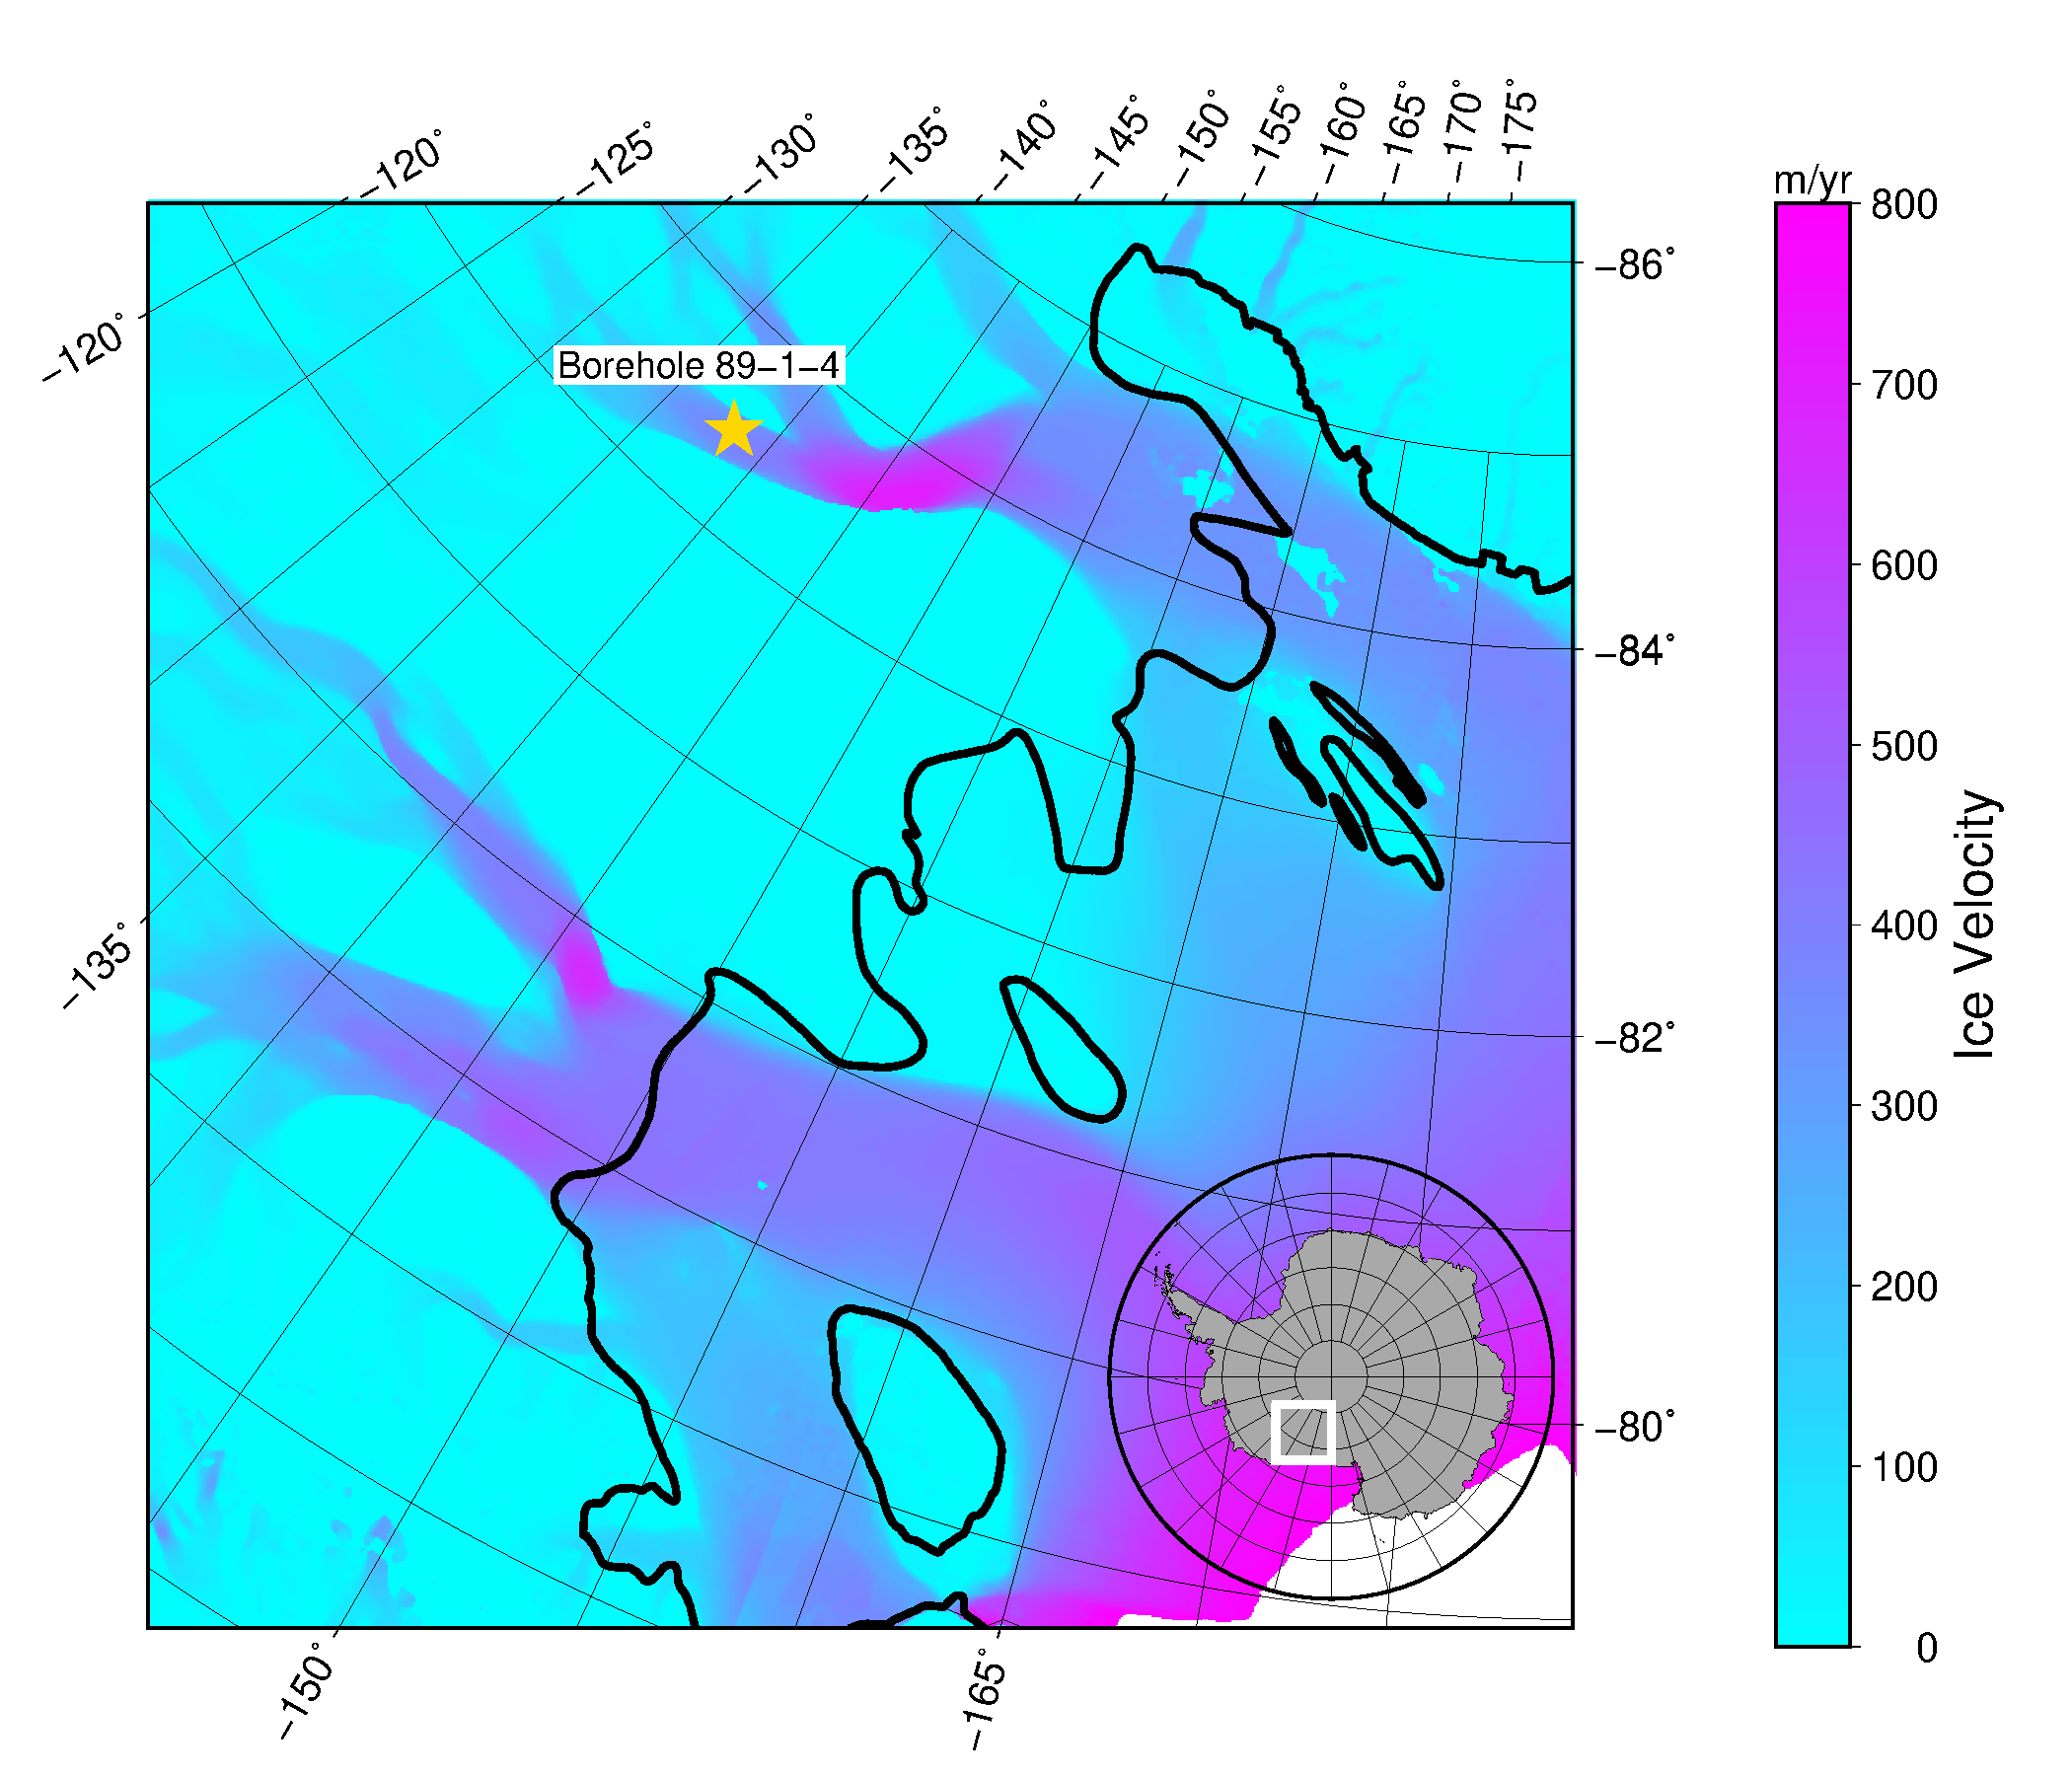
\includegraphics[scale=0.4]{chap_whillans/Figure1.pdf}
   	\caption{Samples for this study were obtained from borehole 89-1-4 near the junction of the B1 and B2 branches of Whillans Ice Stream. Ice velocities of ~600 m/yr are typical in the region [Rignot et al., 2011; Mouginot et al., 2014]. The grounding line is marked in solid black.}
  	\label{}
\end{figure}
% End Figure %

% Figure %
\begin{figure}
	\centering
		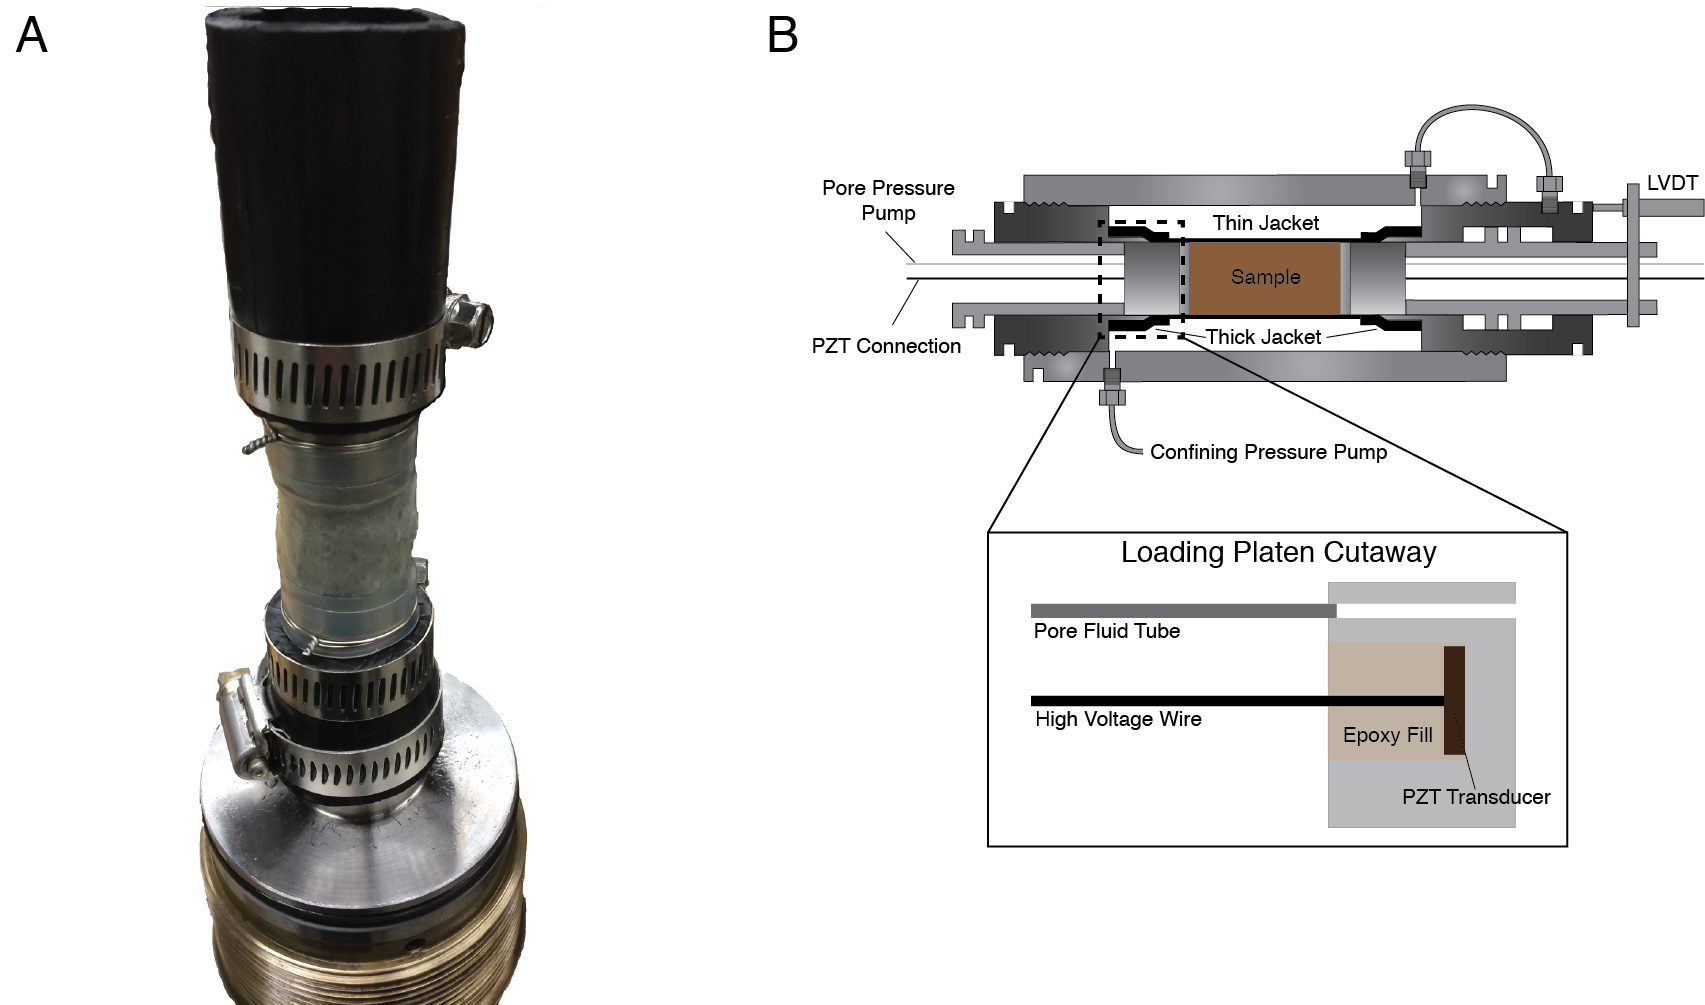
\includegraphics[scale=0.5]{chap_whillans/Figure2.png}
   	\caption{A) The completed sample assembly ready to be loaded into the pressure vessel. B) Schematic diagram of the tri-axial loading cell. Heat shrink tubing was used as a thin, low-strength jacketing material. A hydraulic syringe pump provided isotropic confining and axial loading stresses. A linearly variable displacement transformer (LVDT) measured sample stain. Two high-precision water syringe pumps imposed a hydraulic head to determine sample permeability. Piezoelectric transducers in the loading platens measured the elastic wave travel time through the core (inset). }
  	\label{}
\end{figure}
% End Figure %

% Figure %
\begin{figure}
	\centering
		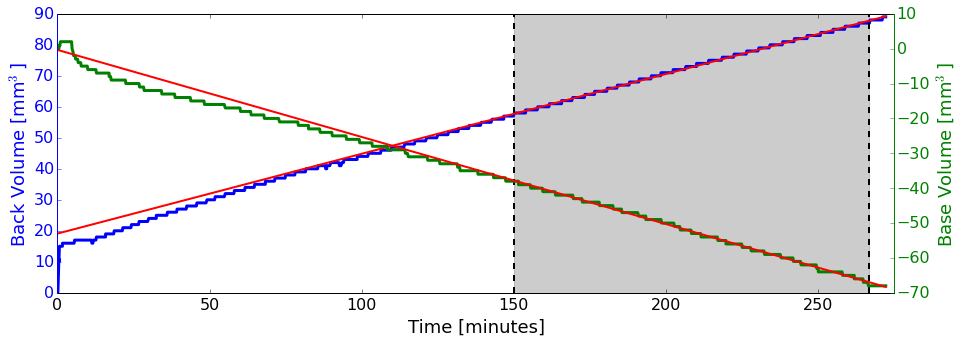
\includegraphics[scale=0.45]{chap_whillans/Figure3.png}
   	\caption{To determine permeability, flow rates from the upstream (blue) and downstream (green) pumps are fit with a least squares fit (red) when the steady-state flow condition is achieved (shaded area). The procedure is repeated at multiple hydraulic heads for repeated permeability measurement.}
  	\label{}
\end{figure}
% End Figure %

\clearpage

% Figure %
\begin{figure}
	\centering
		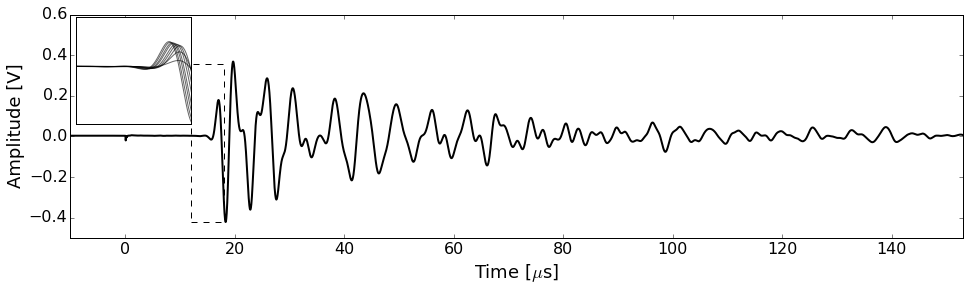
\includegraphics[scale=0.45]{chap_whillans/Figure4.png}
   	\caption{An example acoustic waveform collected during the step-loading test. Inset shows changes in travel time with step loading to 1 MPa effective stress. First arrivals are picked with a cross-correlation technique for consistency. }
  	\label{}
\end{figure}
% End Figure %

% Figure %
\begin{figure}
	\centering
		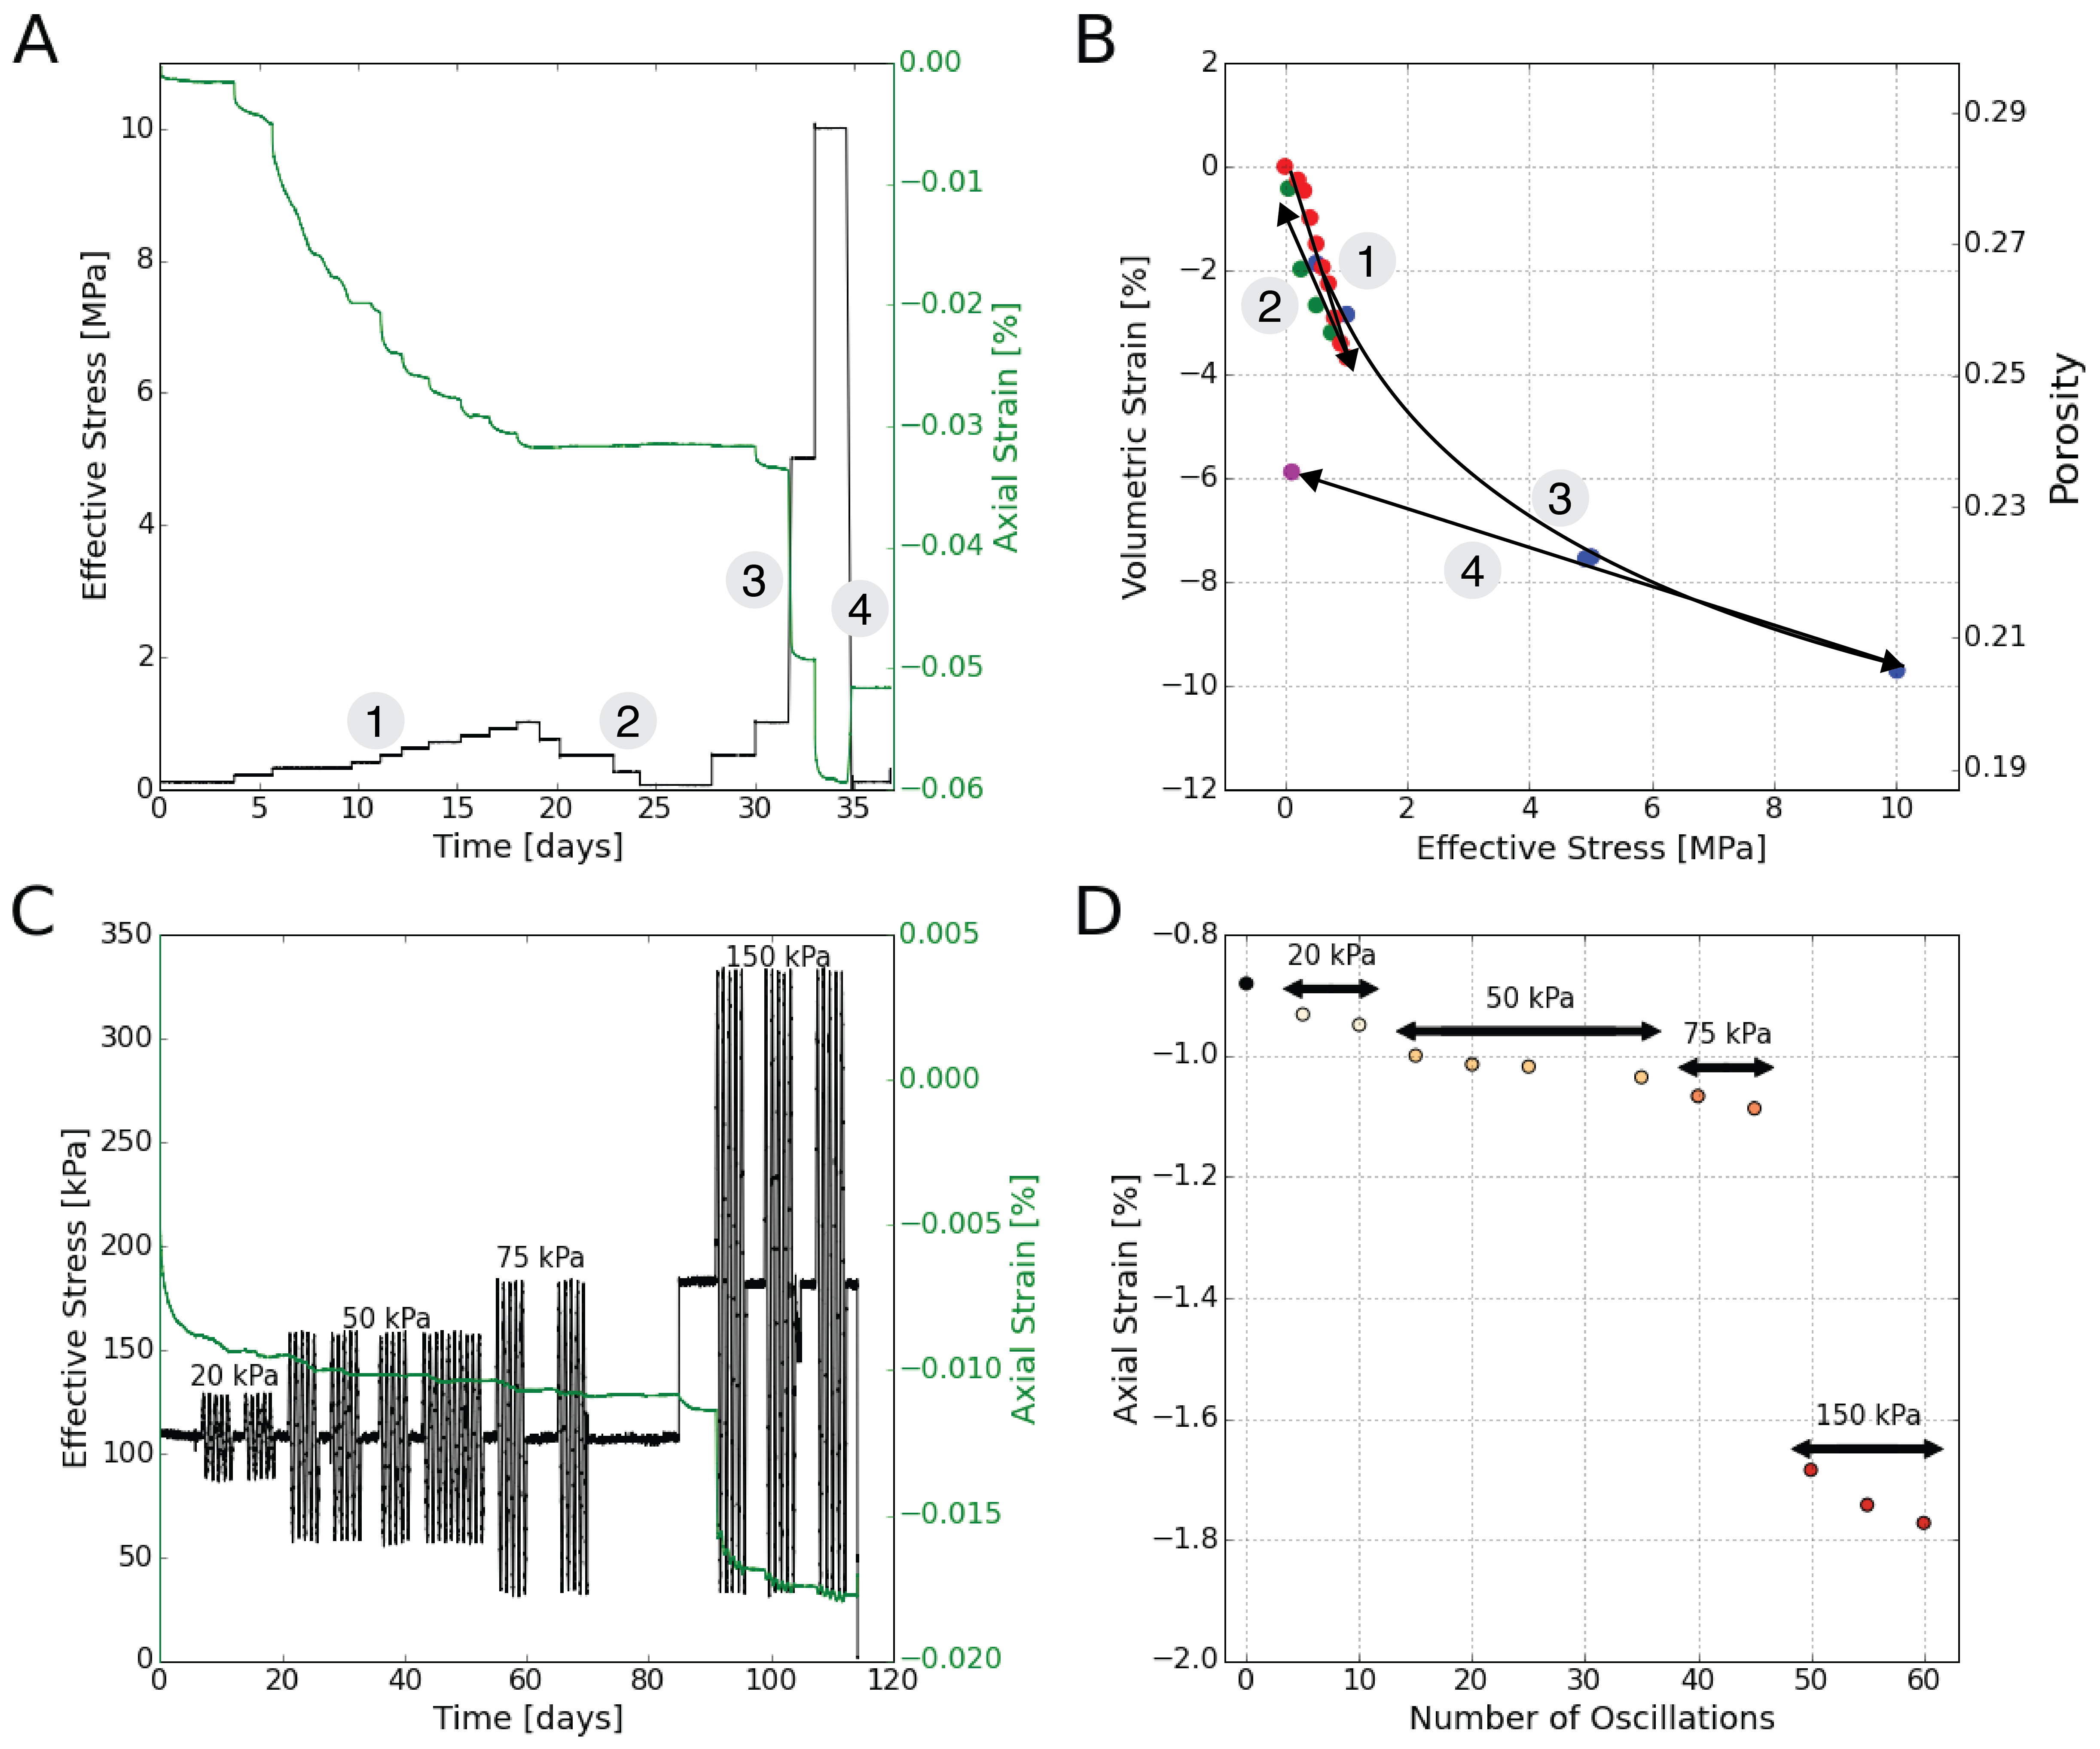
\includegraphics[scale=0.3]{chap_whillans/Figure5.png}
   	\caption{A) Results of the isotropic step loading test show an expected compaction behavior. B) Effective stress and volumetric strain relationship. Initial loading (1) and unloading (2) shows near elastic recovery. Reloading to a 10MPa effective stress (3) created considerable permanent deformation upon the final unloading cycle (4). C) Evolution of axial strain during repeated tidal load cycling. All cycles had a 24-hour period with amplitudes of +/- 25, 50, 75, and 150 kPa. D) Strain was accumulated during all cycle sets, but the additional observed strain decreased with each subsequent set until the amplitude was increased.}
  	\label{}
\end{figure}
% End Figure %

% Figure %
\begin{figure}
	\centering
		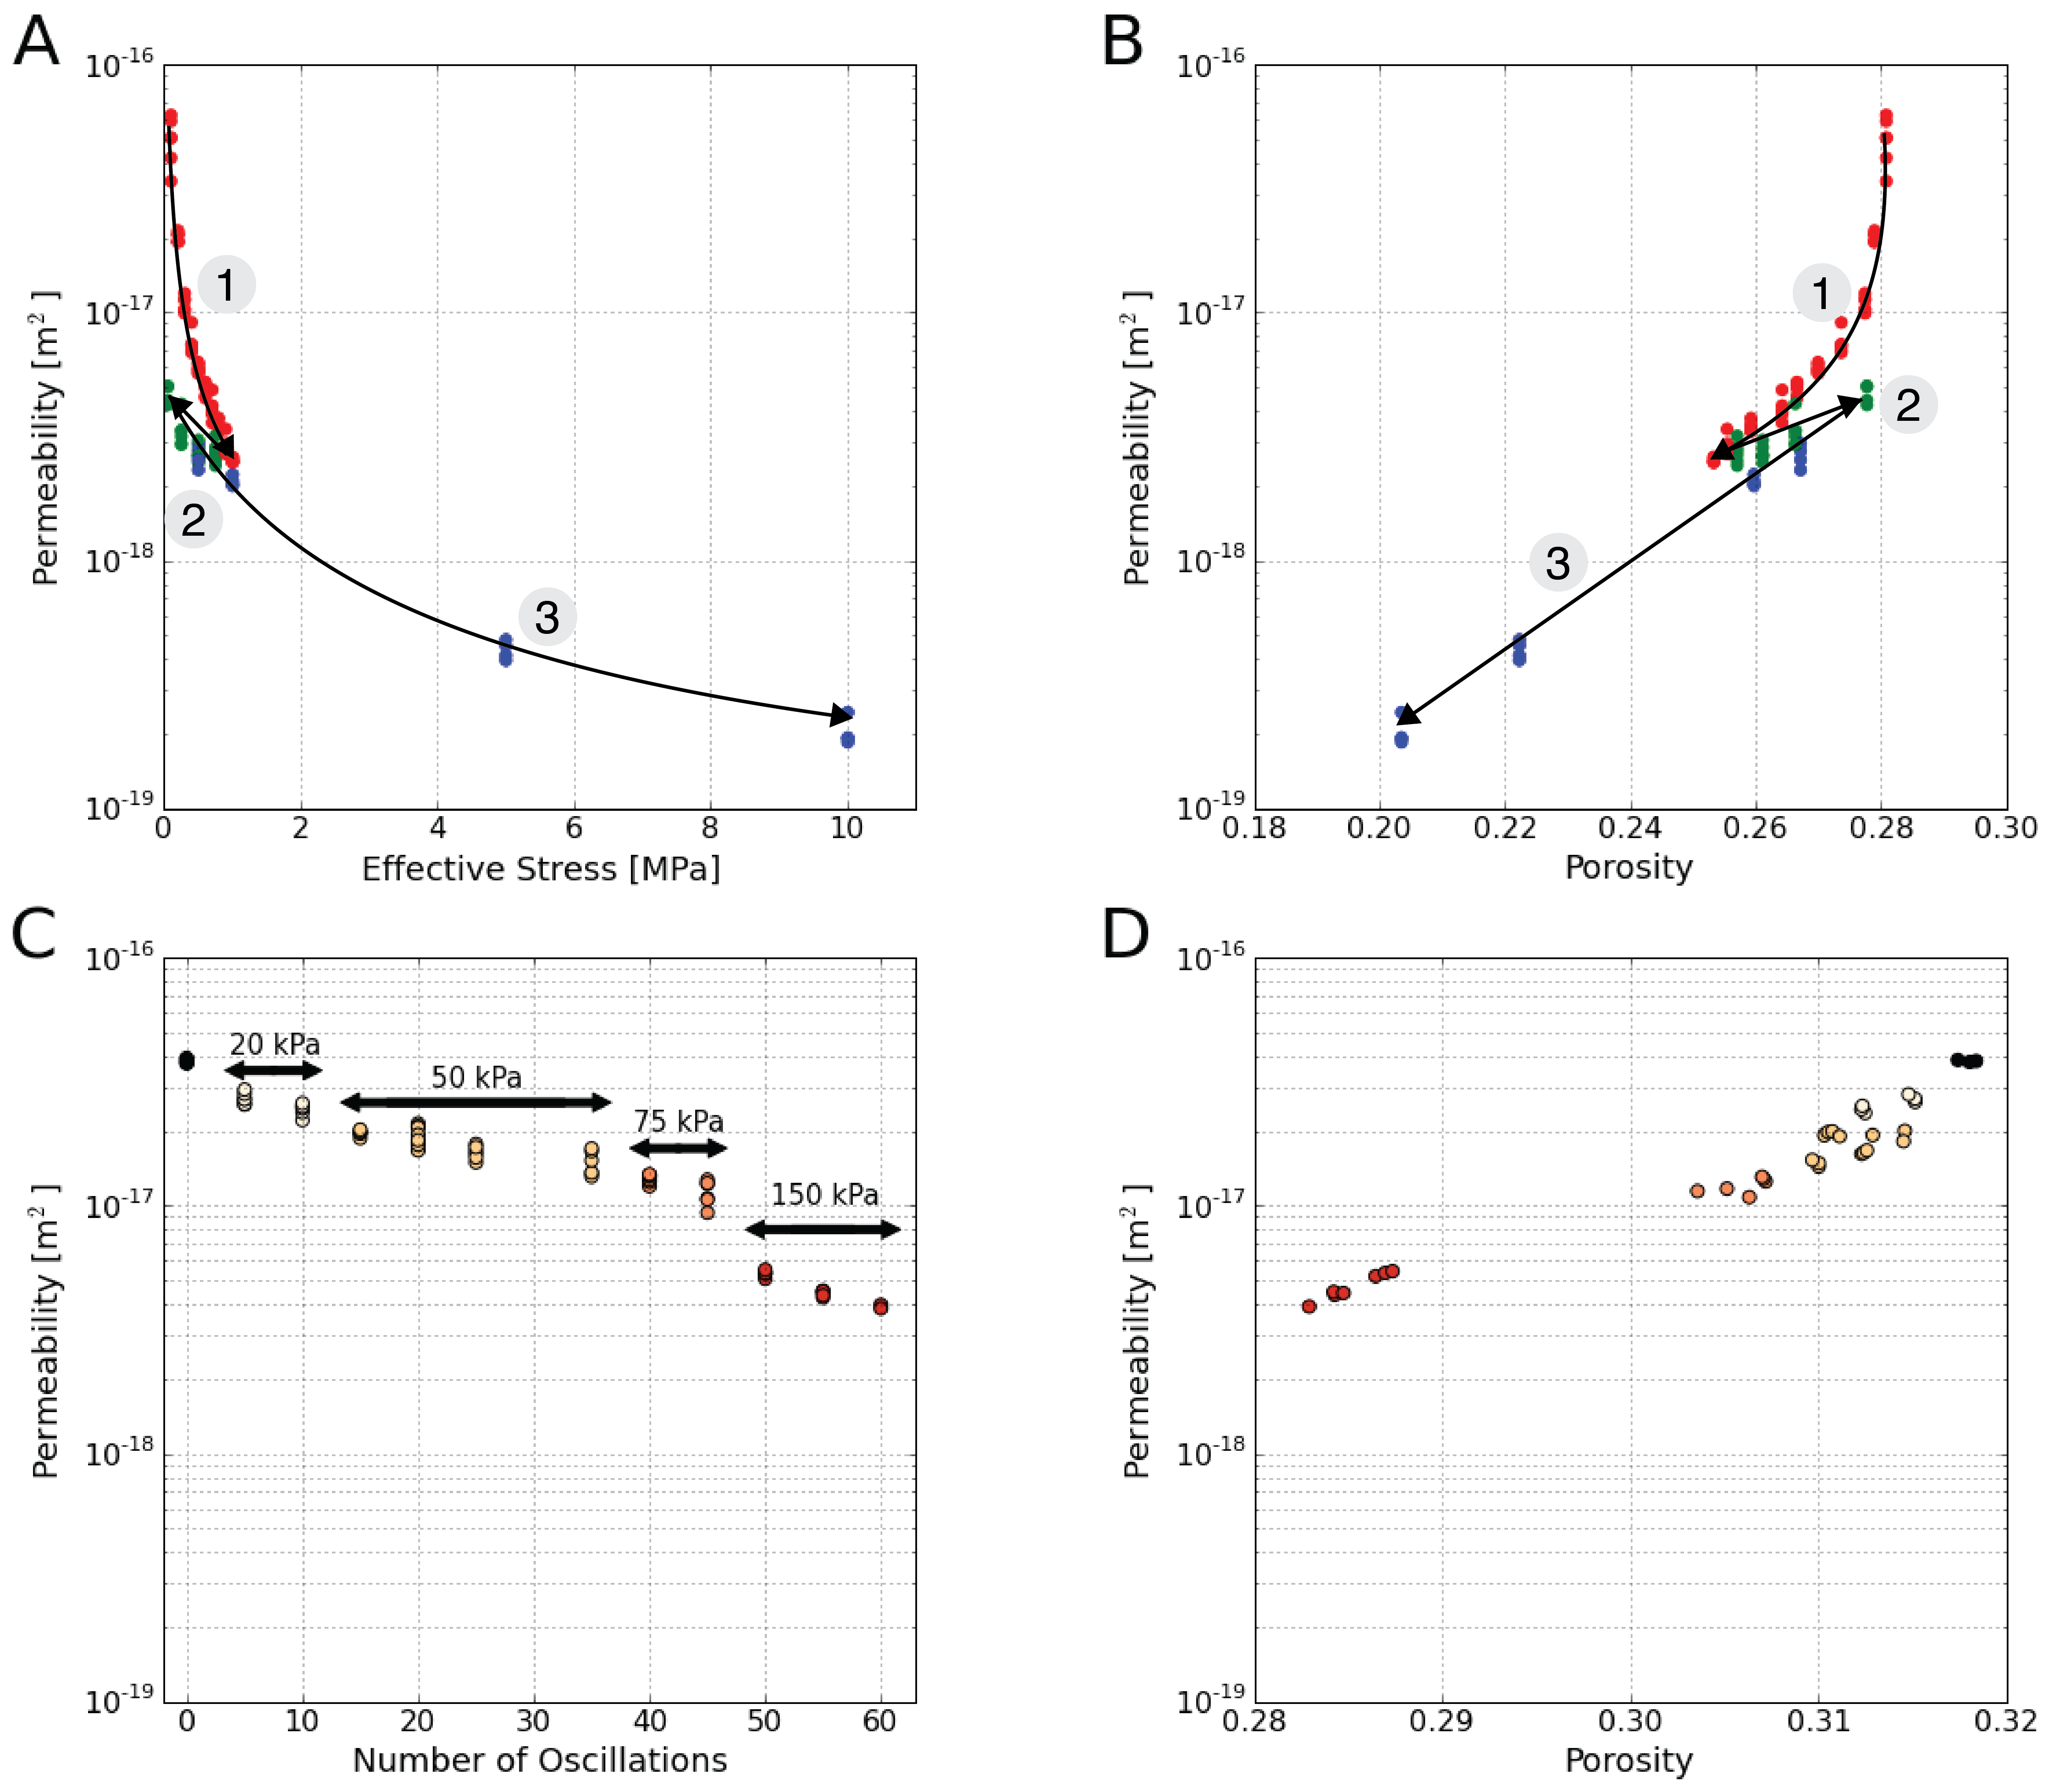
\includegraphics[scale=0.3]{chap_whillans/Figure6.png}
   	\caption{A) Permeability evolution during the step-loading test. Initial permeability values of approximately 3.5�10-17 m2 were reduced by over an order of magnitude during the initial loading (1) with little recovery upon unloading (2). Permeability was reduced by an order of magnitude during reloading (3) to an effective stress of 10 MPa. B) Initial porosity values of 28\% are lower than field estimates. The trend mirrors that of volumetric strain. C) Evolution of permeability and porosity during the tidal loading test indicate that both can be significantly reduced with little additional loading stress, but with load cycling. Initial porosity of 32\% was reduced by several percent over the 60 simulated tidal cycles. D) Permeability was also reduced by an order of magnitude during the cycling. All measurements shown were taken after cycling was complete and the sample had equilibrated.}
  	\label{}
\end{figure}
% End Figure %

% Figure %
\begin{figure}
	\centering
		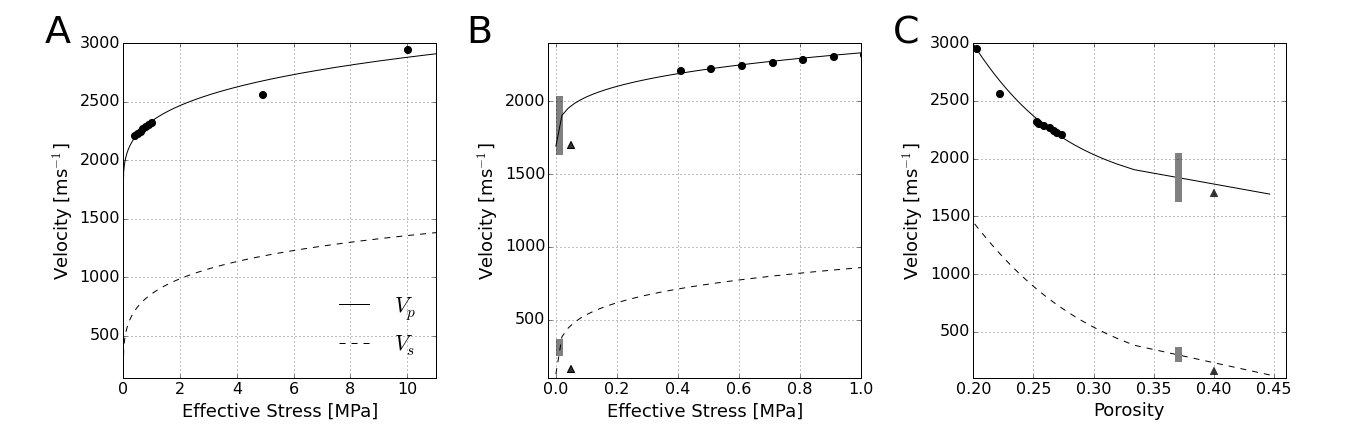
\includegraphics[scale=0.33]{chap_whillans/Figure7.png}
   	\caption{(A) Predicted compressional and shear wave velocities from the effective medium model as a function of effective stress, (B) an expanded view showing field velocity measurements from seismic experiments, and porosity (C). The model is supported by experimental compressional wave velocity measurements, but no shear wave measurements could be obtained in the laboratory due to the very low effective pressures of the experiment. Black circles represent direct measurements from the laboratory, gray bars are velocity estimates by Luthra et al. [2016] and black triangles are estimates by Blankenship et al. [1987].}
  	\label{}
\end{figure}
% End Figure %

\clearpage

% Figure %
\begin{figure}
	\centering
		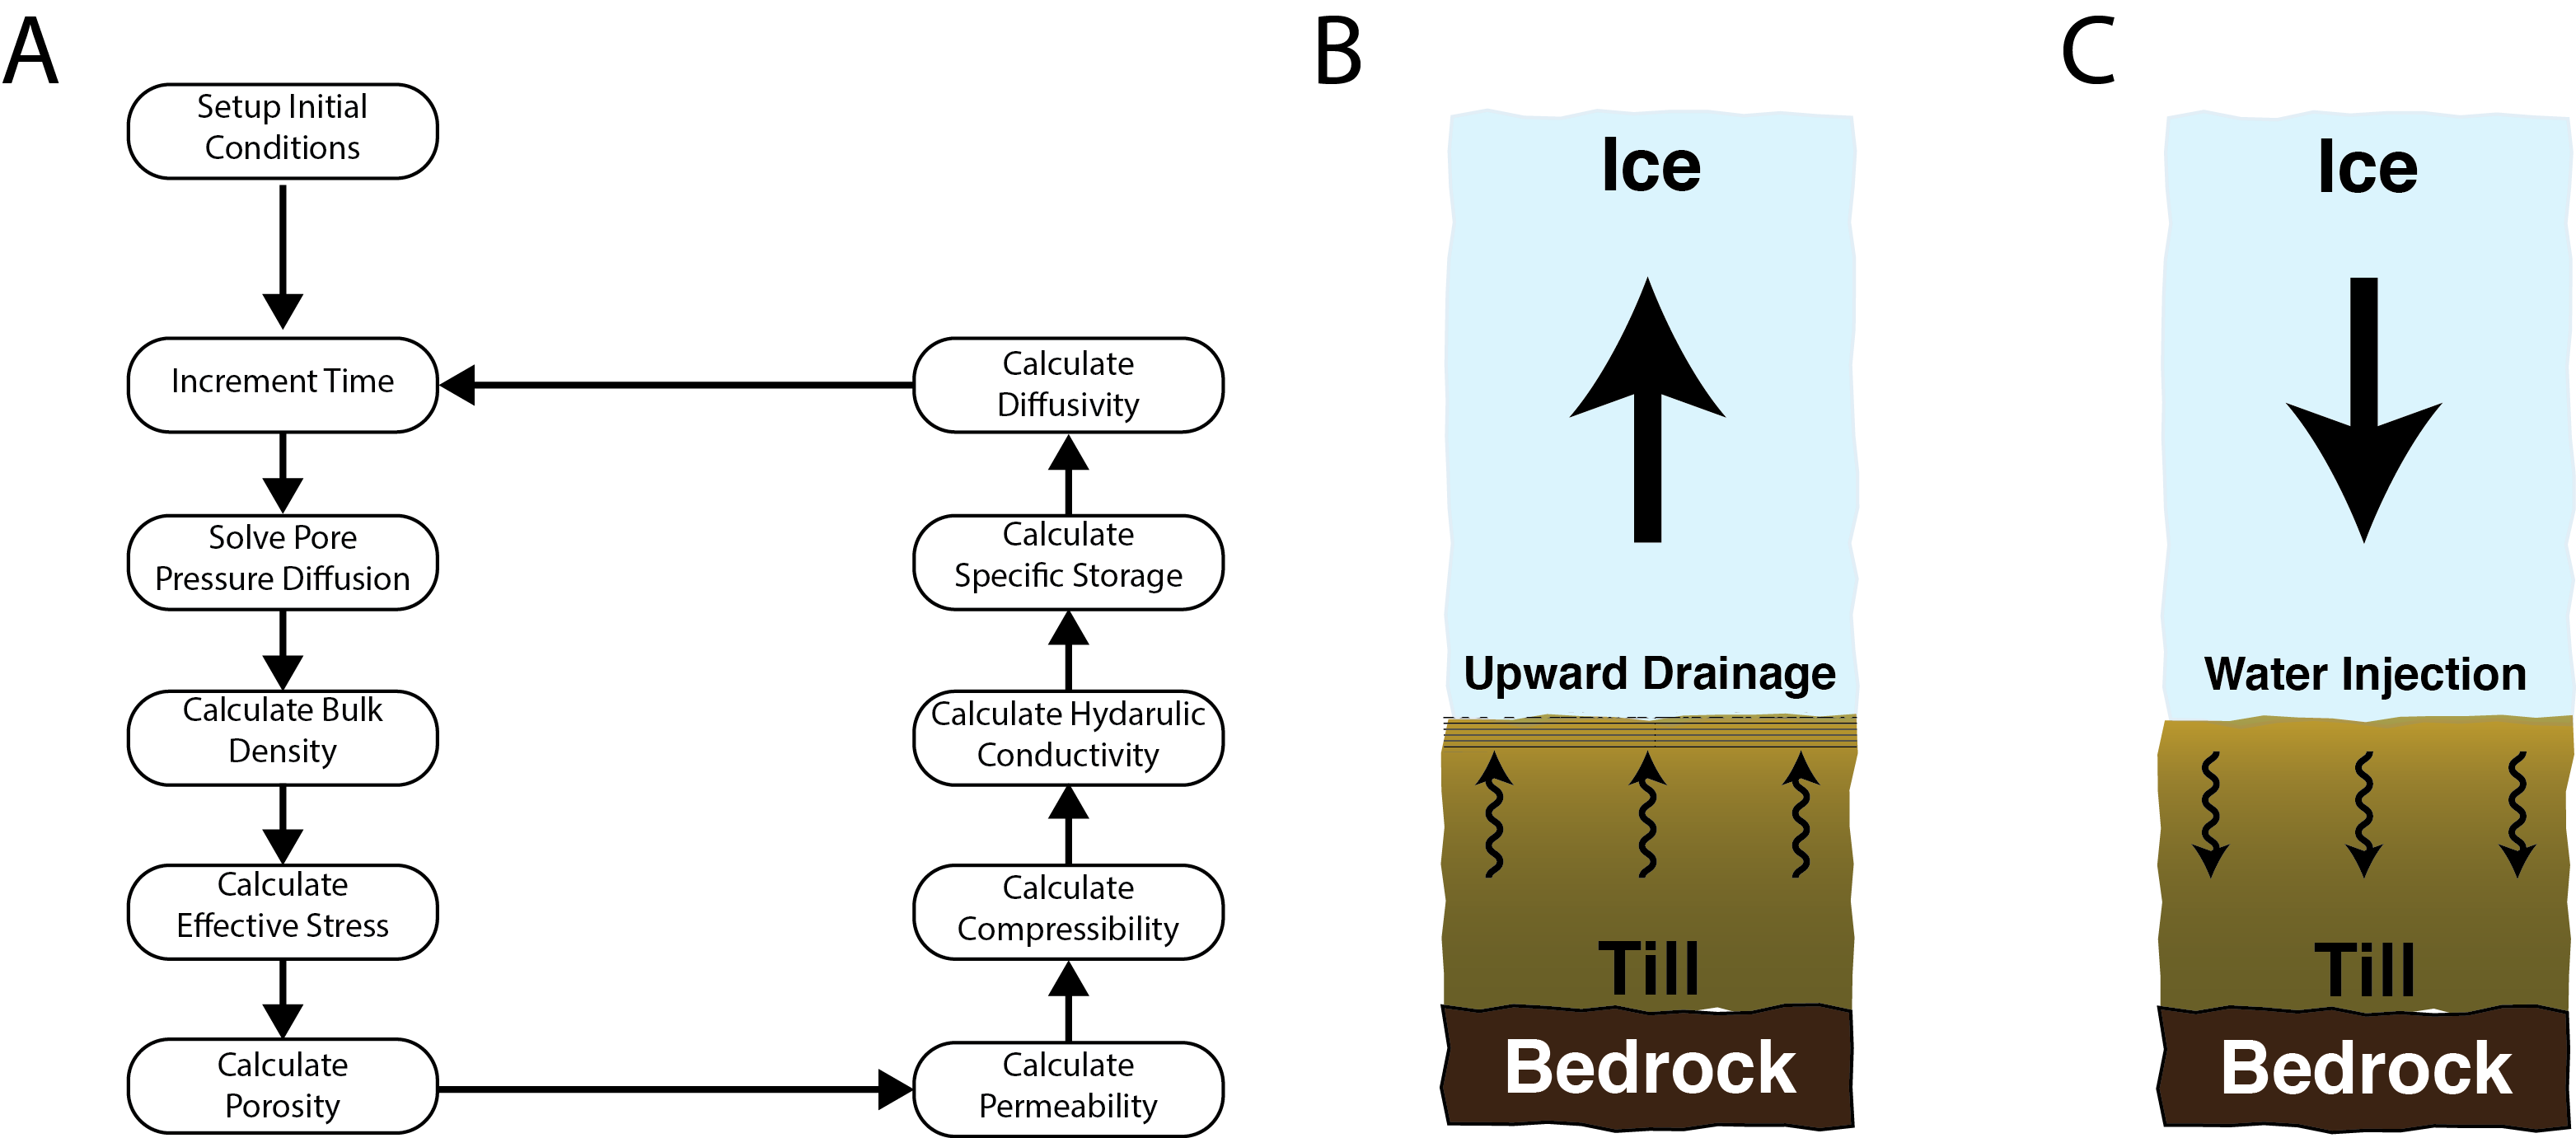
\includegraphics[scale=0.5]{chap_whillans/Figure8.png}
   	\caption{A) Flow chart showing the sequence used when computing the 1-D hydrologic model. B) A cartoon version of the system with ice unloading the till beneath it on a tidal timescale. Upward drainage as a result of lower effective stress at the ice-till interface will quickly result in the formation of a hard layer that slows further drainage and limits the hard layer depth to tens of centimeters. C) Loading from the ice will inject water back into the till as the basal hydraulic pressure is increased.}
  	\label{}
\end{figure}
% End Figure %

\clearpage

% Figure %
\begin{figure}
	\centering
		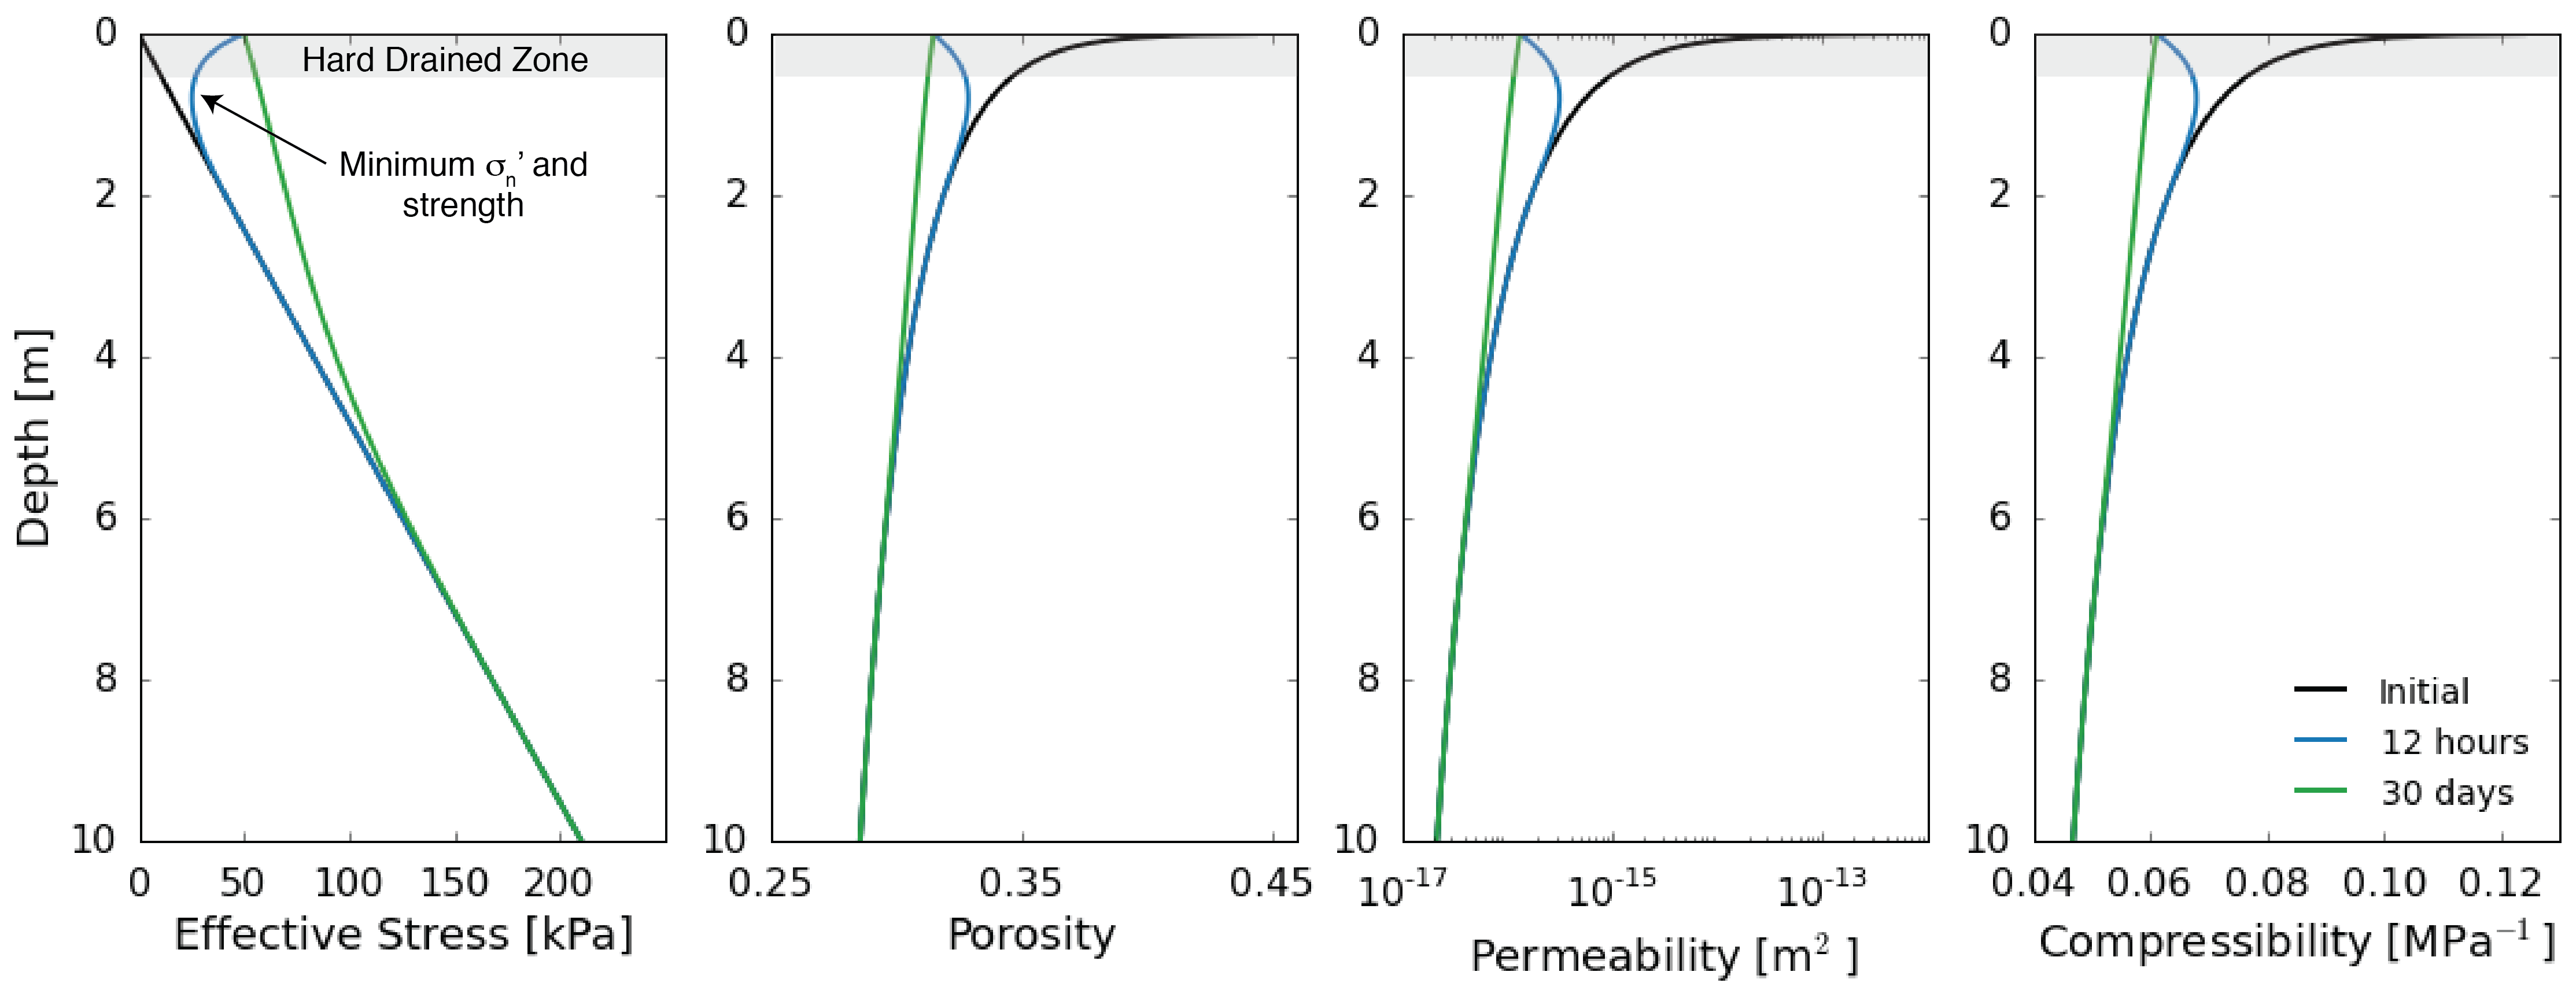
\includegraphics[scale=0.4]{chap_whillans/Figure9.png}
   	\caption{Model results for a coupled diffusion/compaction model of the till layer with an imposed 50 kPa effective stress perturbation at the top boundary.  The perturbation can affect the till over several tens of centimeters in a 12 hour tidal time scale. Over a longer perturbation, such as moving over a rough area on the bed, the till can come close to equilibrium in a month. }
  	\label{}
\end{figure}
% End Figure %

% Figure %
\begin{figure}
	\centering
		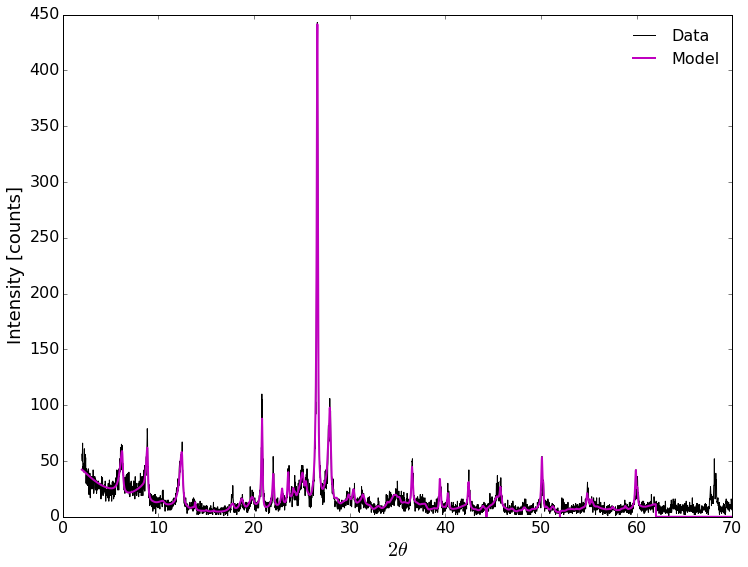
\includegraphics[scale=0.5]{chap_whillans/FigureS1.png}
   	\caption{XRD analysis shows very high clay content in the till samples with significant amounts of quartz as well. Some non-uniqueness exists in the type of clays present, but an effort was made to minimize the misfit with reasonable geological constraints.}
  	\label{}
\end{figure}
% End Figure %

\clearpage

% Figure %
\begin{figure}
	\centering
		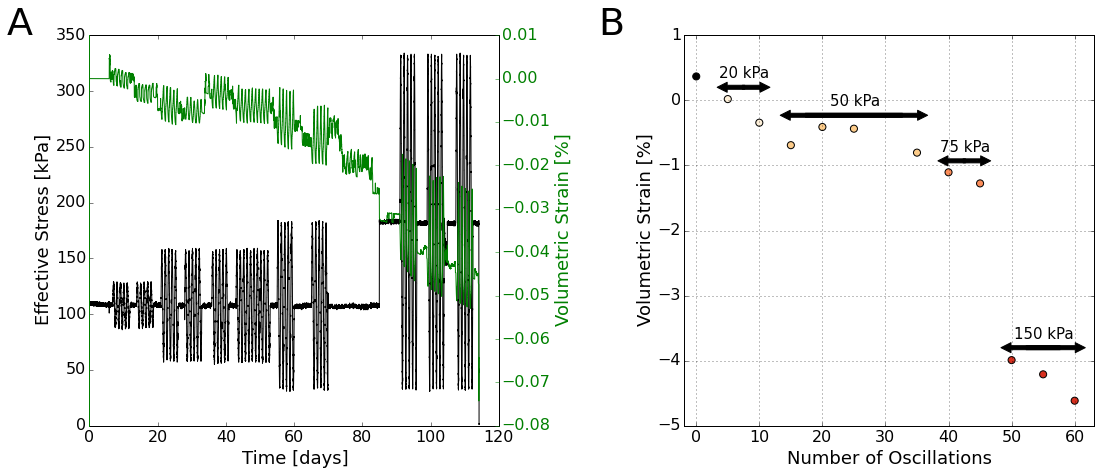
\includegraphics[scale=0.33]{chap_whillans/FigureS2.png}
   	\caption{A) Evolution of volumetric strain during repeated tidal load cycling. B) Strain was accumulated during all cycle sets, similar to the axial strain trends, but with some slight anomalies likely induced by thermal effects on pump volume measurements as volume changes are very small.}
  	\label{}
\end{figure}
% End Figure %

\clearpage

% Figure %
\begin{figure}
	\centering
		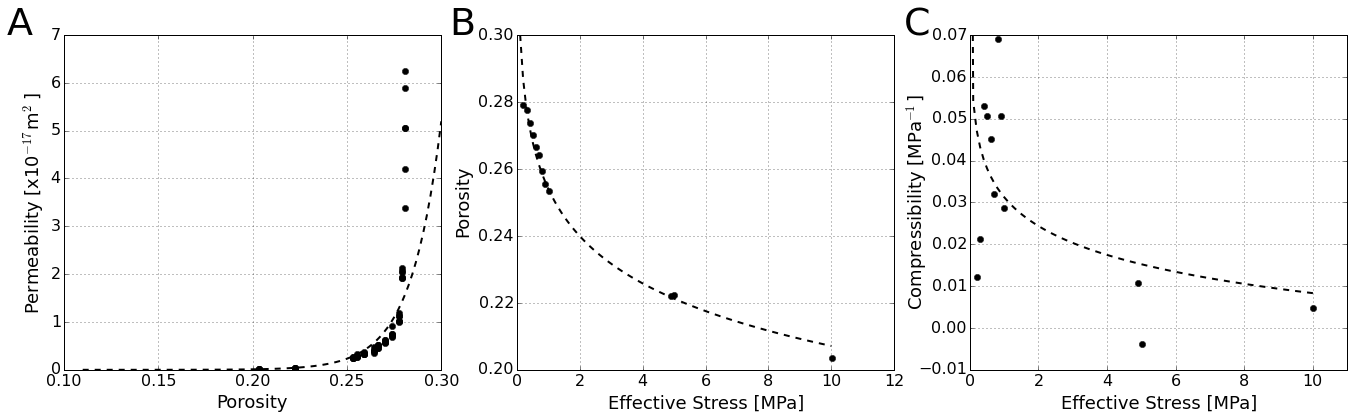
\includegraphics[scale=0.3]{chap_whillans/FigureS3.png}
   	\caption{Experimental data and fits used in loading portions of the simple hydrologic model. Porosity-permeability (A) was fit with an exponential, while effective stress - porosity (B) and effective stress - compressibility (C) were fit with logarithmic relationships.}
  	\label{}
\end{figure}
% End Figure %

\clearpage

\begin{table*}
    \begin{tabular}{|c|c|c|c|c|}
    \hline
    Mineral & Volume Percent & Bulk Modulus [GPa] & Shear Modulus [GPa] & Density [kg/m3]\\
\hline
Quartz & 23.73 & 36.6 & 45 & 2650\\
\hline
Clay & 50.49 & 48 & 20 & 2626\\
\hline
Feldspar & 25.78 & 76 & 26 & 2560\\
    \hline
    \end{tabular}
    \caption{Physical parameters used to construct the effective medium model of compressional and shear wave velocities. Values are based on Dvorkin [1999] and Wang [2001].
}
\end{table*}











